\documentclass[a4paper,12pt]{article}

\usepackage[pdftex]{graphicx}
\usepackage{amsmath,amsfonts,amsthm}
\usepackage{fullpage}

\newtheorem{lemma}{Lemma}

\newcommand{\grid}[4]{ %
	\begin{tabular}{|c|c|} %
		\hline %
		#1 & #2 \\
		\hline %
		#3 & #4 \\
		\hline %
	\end{tabular} %
}

\author{April Camp 2017}
\title{Test 1 -- Solutions}
\date{}

\begin{document} \maketitle

\begin{enumerate}
	\item 
	\textit{Determine all positive integers $k$ and $n$ satisfying the equation \[k^2 - 2016 = 3^n.\]}
	Note that if $n \geq 3$, then modulo $27$ the equation becomes $k^2 \equiv
	18 \pmod{27}$, which is a contradiction since $18$ is not a quadratic residue
	modulo $27$. Thus the only possible solutions correspond to $n=1$ and
	$n=2$. For $n=1$, the equation becomes $k^2 = 2019$, and for $n=2$, the
	equation is $k^2 = 2025 = 45^2$. We see that the only solution in
	positive integers is given by $n=2$ and $k=45$.
		
	\item 
	\textit{Let $ABC$ be an acute angled triangle. Let $H$ be the foot of the altitude from $C$ onto $AB$. Suppose that $|AH|=3|BH|$. Let $M$ and $N$ be the midpoints of the segments $AB$ and $AC$ respectively. Let $P$ be a point such that $|NP|=|NC|$ and $|CP|=|CB|$ and such that $B$ and $P$ lie on opposite sides of the line $AC$. Show that $\angle APM = \angle PBA$.}
	
	{\centering 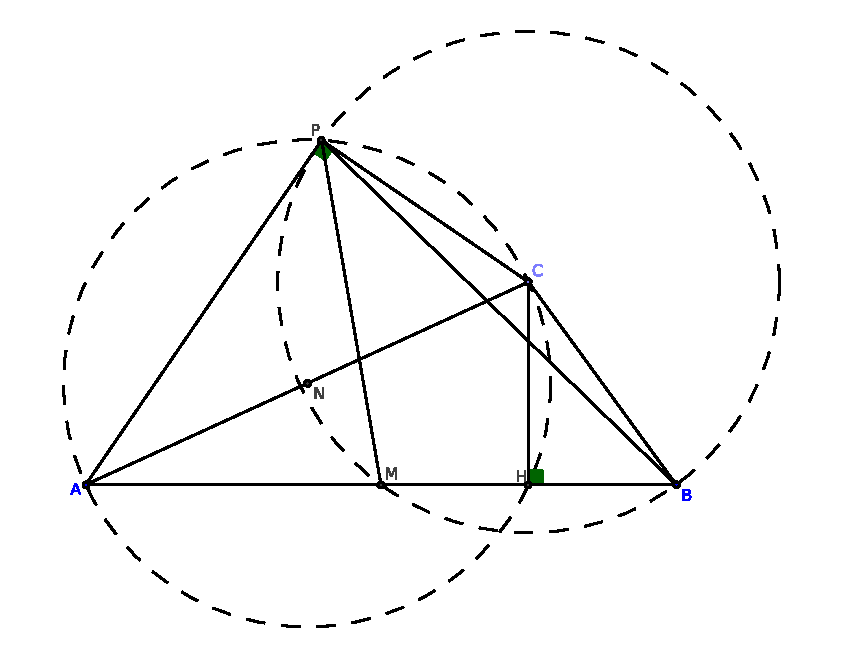
\includegraphics[width=0.9\textwidth]{T1Q2.eps}}
	
	Note that since $HB =\frac{1}{4}AB =\frac{1}{2}MB$ and $CH \perp MB$, $CH$ is the perpendicular bisector of $MB$ and so $CM=CB=CP$. Thus $P$, $B$ and $M$ lie on a circle centred at $C$, which we call $\Gamma$. Also, since $N$ is the midpoint of $AC$ and $NC=NP$, $P$ lies on the with diameter $AC$, centred at $N$. So $AP \perp PC$, and so $AP$ is tangent to $\Gamma$. Thus by the tan-chord theorem, $\angle APM =\angle PBM =\angle PBA$.
	
	\item
	\textit{Consider a $4 \times 4$ grid of unit squares. How many ways are there to write a 0 or 1 in each $1 \times 1$ square so that the product of the two numbers written on every neighbouring pair of squares (sharing a common edge) is always 0?}
	
	Suppose that we have a collection of tiles, and in each tile is written
	either a $0$ or a $1$. We will call this configuration of tiles
	\emph{valid} if it satisifies the condition imposed in the problem:
	whenever two tiles share a border, the product of the numbers written
	in these two tiles is $0$. We wish to count the number of valid $4 \times
	4$ grids of tiles. We first prove two lemmas about the number of valid
	assignments of numbers to tiles in certain configurations.

	\begin{lemma} \label{lemma:strip}
		Let $a_n$ be the number of valid assignments of numbers to $n$ tiles
		placed in a line. (i.e. a $1 \times n$ strip of tiles.) Then $a_n =
		F_{n+2}$, where $F_n$ is the $n^\text{th}$ Fibonacci number.
	\end{lemma}
	\begin{proof}
		for $n=0$, there is $1$ valid assignment. (The ``empty
		assignment"), and for $n=1$, there are $2$ valid assignments. Thus
		$a_0=F_2$ and $a_1=F_3$. We now show that $a_{n} = a_{n-1} + a_{n-2}$,
		which then establishes the claim.

		Consider the number placed in the final tile in the strip. If it is a
		$0$, then we can place any numbers in the remaining tiles as long as
		the remaining $1 \times (n-1)$ strip is valid, and so there are
		$a_{n-1}$ valid configurations in this case. If the number in the final
		tile is a $1$,
		then this forces the penultimate tile to contain a $0$, and there
		are then no other restrictions other than that the remaining $1 \times
		(n-2)$ strip of tiles is valid. There are thus $a_{n-2}$ ways to validly
		assign the numbers in this case, and so we find that $a_n = a_{n-1} +
		a_{n-2}$.
	\end{proof}

	\begin{lemma} \label{lemma:ring}
		Let $b_n$ be the number of valid assignments of numbers to $n$ tiles
		fixed to a wall in a ring pattern. (i.e. the border of a rectangle.) Then
		$b_n = a_{n-1} + a_{n-3} = F_{n+1} + F_{n-1}$ for all $n \geq 4$.
	\end{lemma}
	\begin{proof}
		Consider any tile in the ring. If it contains a $0$, then the rest of
		the ring is a (bent) valid $1 \times (n-1)$ strip of tiles, and so we
		have that there are $a_{n-1}$ valid configurations in this case. On the
		other hand, if the chosen tile contains a $1$, then the two tiles
		which border it must both contain a $0$, and the remaining $(n-3)$
		tiles in the ring is now just any valid $1 \times (n-3)$ strip of
		tiles, and so there are $a_{n-3}$ valid configurations in this case.
	 
		We see that $b_n = a_{n-1} + a_{n-3}$, and by Lemma \ref{lemma:strip},
		this is equal to $F_{n+1} + F_{n-1}$.
	\end{proof}

We now return to the problem. We consider three cases based on the number
of $0$'s contained in the central $2 \times 2$ subgrid of squares.

\begin{enumerate}

	\item[Case 1:] Four $0$'s: \grid{0}{0}{0}{0}
		
		Consider the ring of $12$ squares surrounding the central $2 \times
		2$ subgrid. The board as a whole is valid precisely when these $12$
		squares are, and so by Lemma \ref{lemma:ring}, we find that there
		are thus $F_{11} + F_{13} = 89 + 233 = 322$ valid grids in this case.

	\item[Case 2:] Three $0$'s: \grid{0}{0}{0}{1} \grid{0}{0}{1}{0}
		\grid{0}{1}{0}{0} \grid{1}{0}{0}{0}

		In this case, the squares on the border adjacent to the central square
		with a $1$ in must contain $0$'s. The square on the border which shares
		a corner with the square with a $1$ in can then be either a $1$ or a
		$0$, and in each of these cases, the remaining $9$ squares on the
		border can be any of the $a_9 = F_{11} = 89$ possible $1 \times 9$
		strips of valid tiles. In each of the $4$ configurations for the central
		$2 \times 2$ subgrid, we thus have $2 \times 89 = 178$ possible valid
		grids, giving us $178 \times 4 = 712$ valid configurations in this
		case.

	\item[Case 3:] Two $0$'s: \grid{0}{1}{1}{0} \grid{1}{0}{0}{1}

		The squares on the border adjecent to the $1$'s must be filled with
		$0$'s. The squares on the border sharing a corner with the $1$'s can be
		filled in any any way. For each of the $4$ possible ways of filling
		these squares, the remaining border squares form two independent $1
		\times 3$ strips of tiles, which can each be filled in $a_3 = F_5 =
		5$ ways, and so we see that the number of valid
		configurations in this case is $2 \times 4 \times 5^2 = 200$.

\end{enumerate}

Combining the above three cases, we find that the total number of valid $4
\times 4$ grids is given by $322 + 712 + 200 = 1234$.

	\item 
	\textit{Find all functions $f:\mathbb{R} \rightarrow \mathbb{R}$ satisfying $$f(xy-1)+f(x)f(y) = 2xy - 1$$ for all $x,y \in \mathbb{R}$.}
	
	We call the above equation Rosa. Note that if $f$ is a constant function, then the left-hand side of Rosa is constant as $x$ and $y$ vary, while the right-hand side is obviously not. Hence $f$ is nonconstant. Putting $y=0$ in Rosa, we see that $f(-1) +f(0)f(x) = -1$ for all $x\in\mathbb{R}$. Since $f$ is nonconstant, we must have that $f(0)=0$, and consequently $f(-1) = -1$. Also, putting $x=y=1$ in Rosa we get that $f(1)^2 = 1$, so $f(1) = 1$ or $f(1) = -1$.
	
	Now putting $y = -1$ in Rosa we get that $-2x-1 = f(-x-1) +f(x)(f-1) = f(-x-1)-f(x)$, putting $y=1$ in Rosa we get that $f(x-1) +f(1)f(x) = 2x-1$, and putting $y=x$ in Rosa we get that $f(x^2-1) +f(x)^2 = 2x^2-1$.
	\begin{align*} \text{Now } f(z)f(y) &= 2zy-1-f(zy-1) = 2(-zy)(-1) -1 -f((-zy)(-1)-1) \\ &= f(-zy)f(-1) = -f(-zy) \quad \text{ for all } z,y\in\mathbb{R}.\end{align*}
	Putting $z=x-1$ and $y=-x-1$ in this equation, we get that
	\begin{align*} f(x-1)f(-x-1) &= -f(x^2-1) \\
		\iff [2x-1-f(1)f(x)] [f(x)-2x-1] &= -[2x^2-1-f(x)^2] = f(x)^2 -2x^2 +1.
	\end{align*}
	Now if $f(1)=1$, this equation becomes \begin{align*} f(x)^2 -2x^2 +1 &= (1+2x-f(x))(1-2x+f(x)) \\ &= 1 -(2x-f(x))^2 = 1 -4x^2 +4xf(x) -f(x)^2 \\ \iff 0 &= 2x^2 -4xf(x) -2f(x)^2 = -2(f(x)-x)^2 \\ f(x) &= x \quad \text{for all } x\in\mathbb{R}. \end{align*}
	On the other hand, if $f(1) = -1$, the equation becomes
	\begin{align*} f(x)^2 -2x^2 +1 &= (f(x)-1-2x)(f(x)-1+2x) \\ &= (f(x)-1)^2 -(2x)^2 = f(x)^2-2f(x)+1-4x^2 \\ \iff 2f(x) &= -2x^2 \\ \iff f(x) &= -x^2 \quad \text{for all } x\in\mathbb{R}. \end{align*}
	
	So we see that $f(x)=x$ and $f(x)-x^2$ are the only possible solutions. Now it remains to check that both of these are valid solutions by plugging them into Rosa. For $f(x)=x$, $f(xy-1) +f(x)f(y) = xy-1-xy = 2xy-1$, so the solution checks. For $f(x)=-x^2$, $f(xy-1) +f(x)f(y) = -(xy-1)^2 +(-x^2)(-y^2) = -x^2y^2 +2xy -1 +x^2y^2 = 2xy-1$, so this solution also checks. Hence all the possible solutions to this functional equation are $f(x)=x$ for all $x\in\mathbb{R}$ and $f(x)=-x^2$ for all $x\in\mathbb{R}$.
	
	\item
	\textit{Find all infinite sequences $a_1, a_2, a_3 \dots $ of positive integers such that
	\begin{itemize}
	\item [(a)] $a_{mn} = a_ma_n$ for all positive integers $m$ and $n$, and
	\item [(b)] there are infinitely many positive integers $n$ such that $$\{1, 2, \dots, n\} = \{a_1, a_2, \dots, a_n \}.$$
	\end{itemize}}
	
	
	
\end{enumerate}

\end{document}
